\subsection{Multiply}
\label{subsection:multiply}

\begin{figure}[!h]
\begin{center}
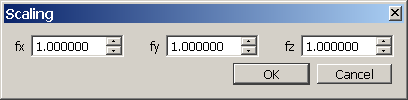
\includegraphics[width=0.4\textwidth]{Partie3_Fonctions/Multiply.png}
\caption{\label{fig:multiplyDlg}Bo�te de dialogue pour la multiplication des coordonn�es}
\end{center}
\end{figure}

Multiplie les coordonn�es des points des entit�s s�lectionn�es par des constantes.\\
\par
L'utilisateur saisit les 3 coefficients multiplicateurs suivant chaque axe $(f_{X},f_{Y},f_{Z})$ via une bo�te de dialogue (voir~\ref{fig:multiplyDlg}).

